\documentclass{beamer}
\usepackage[utf8]{inputenc}
\usepackage[english]{babel}
\usepackage{amsmath}
\usepackage{amssymb}
\usepackage{fancyhdr}
\usepackage{pgfplots}
\usepackage{setspace}
\usepackage{listings}
\pgfplotsset{compat=1.17} 
\usepackage{enumerate}
\usepackage{algorithm}
\usepackage{algpseudocode}
% \geometry{a4paper} % or letter or a5paper or ... etc
% \geometry{landscape} % rotated page geometry
% \usepackage[margin=2cm]{geometry}
\usepackage{minted}
\usepackage[most]{tcolorbox}
\newtcolorbox{tb}[1][]{%
  sharp corners,
  enhanced,
  colback=white,
  height=6cm,
  attach title to upper,
  #1
}

%These setting will make the code areas look Pretty
\lstset{
	escapechar=~,
	numbers=left, 
	%numberstyle=\tiny, 
	stepnumber=1, 
	firstnumber=1,
	%numbersep=5pt,
	language=C,
	% stringstyle=\itfamily,
	%basicstyle=\footnotesize, 
	showstringspaces=false,
	frame=single,
  upquote=true
}

% created 2022-May-23 %
% Theme choice:
\usetheme{AnnArbor}
% Title page details: 
\title{Memory and Pointers in C}
\author{Jonathan Parlett}
\date{\today}

\begin{document}

% Title page frame
\begin{frame}
    \titlepage
\end{frame}

\begin{frame}{Memory}
	A big part of C is memory management, so lets discusses how memory is relevant to programs.

	\begin{itemize}
		\item Each program has a section of memory allocated to it by the operating system when it is executed. 
		\item If a program attempts to access another programs memory space a segmentation fault occurs and the program is terminated.
		\item The operating system is also a program, and there is a section of memory that is owns.
	\end{itemize}
\end{frame}

\begin{frame}{Stack and Heap}
	Each section of memory allocated to a C program by the operating system is divided into the {\bf Stack} and the {\bf Heap}.

	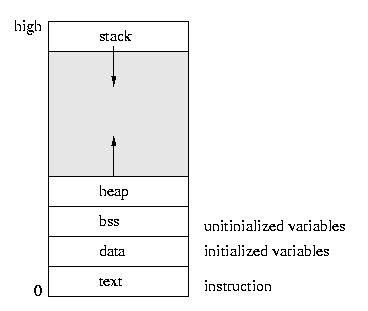
\includegraphics[scale=0.40]{imgs/stackandheap.jpeg}

	Stack memory is managed for you. Whenever you are declaring variables, arrays, or instances of structs, they are located on the stack.
\end{frame}

\begin{frame}{Stack and Heap}
	\begin{itemize}
	\item Anything allocated on the stack is also reclaimed automatically, when the program terminates or things fall out of scope. local variables of a function are reclaimed when the function returns for example.

	\item Whenever you are using {\it malloc()} to get space for a structure or variable you are using memory on the heap. This memory once allocated will not be reclaimed until you reclaim it. It is within your control.
	\end{itemize}
\end{frame}

\begin{frame}{Static vs Dynamic Memory}
	\begin{itemize}
		\item Static or compile time memory is the memory that is managed for you. It again uses the stack. This is managed by the compiler and since items are statically declared in the code we say it is allocated at compile time.

		\item Dynamic memory is again the memory that you manage. It is allocated by calls to {\it malloc()}. So it allocated programmatically during execution execution, so it is also called run time memory allocation.
	\end{itemize}
\end{frame}

\begin{frame}{Memory as a Table}
	We can think of memory as a $n$x2 table. The indices of the table are memory addresses (just numbers), and the data at each row is the value stored in that memory location. For now this is a simplified table. We will ignore the relevance of the sizes of data types, and consider each row a single item of type {\it int}.

	\begin{tabular}{|c|c|}
		\hline
		Address & Data\\
		\hline
		0 & 55 \\
		\hline
		1 & 49 \\
		\hline
		\vdots & \vdots \\
		\hline
		n & 13\\
		\hline
	\end{tabular}

A pointer holds a table index (memory address). So if 49 is stored at location 1 then a pointer to 49 would have the value 1. From this it should be clear that memory addresses are just numbers, so the values of pointers are just numbers. To clarify the value {\bf at} pointers is a different matter, but in C pointers are just 64 bit integers.
\end{frame}

\begin{frame}[fragile]{Pointer Operations: Address Of (\&)}
	Again consider the memory table.

	\begin{tabular}{|c|c|}
		\hline
		Address & Data\\
		\hline
		0 & 55 \\
		\hline
		1 & 49 \\
		\hline
		\vdots & \vdots \\
		\hline
		n & 13\\
		\hline
	\end{tabular}

	Given a data item in our table, the address of (\&) operator gives us the index (memory address) of our data item;

\begin{minted}[frame=lines]{c}
int i = 49; //corresponds to row 1
printf("location of i: %d\n", &i); //prints 1
\end{minted}
In effect {\it \&i} gives us a pointer to {\it i}.

\end{frame}

\begin{frame}[fragile]{Pointer Operations: Dereference (*)}
A pointer holds a table index (memory address). When we dereference said pointer we are retrieving the item at that index.

\begin{tabular}{|c|c|}
		\hline
		Address & Data\\
		\hline
		0 & 55 \\
		\hline
		1 & 43 \\
		\hline
		2 & 8 \\
		\hline
		\vdots & \vdots \\
		\hline
		n & 13\\
		\hline
	\end{tabular}
\begin{minted}[frame=lines]{c}
//pointer holds index 2
int* i = 2;
//dereferencing (*), and printing value at row 2 <-> 8
printf("value at i: %d\n", *i);
\end{minted}
\end{frame}

\begin{frame}[fragile]{Pointer Operations: Addition (+)}
Arrays are one of the most basic data structures, they are simply a collection of contiguous memory locations. So all elements are placed one after the other in memory.
\mint{c}|int A[5] = {1,2,3,4,5}|
Arrays are pointers. The value of $A$ is just a memory address. lets say its 113. Then the array corresponds to the following mem table.
\begin{tabular}{|c|c|}
		\hline
		Address & Data\\
		\hline
		0 & 55 \\
		\hline
		\vdots & \vdots \\
		\hline
		113 & 1\\
		\hline
		114 & 2 \\
		\hline
		115 & 3 \\
		\hline
		116 & 4 \\
		\hline
		117 & 5 \\
		\hline
		\vdots & \vdots \\
		n & 13\\
		\hline
	\end{tabular}

\end{frame}

\begin{frame}[fragile]{Pointer Operations: Addition (+)}
\begin{tabular}{|c|c|}
		\hline
		Address & Data\\
		\hline
		0 & 55 \\
		\hline
		\vdots & \vdots \\
		\hline
		113 & 1\\
		\hline
		114 & 2 \\
		\hline
		115 & 3 \\
		\hline
		116 & 4 \\
		\hline
		117 & 5 \\
		\hline
		\vdots & \vdots \\
		n & 13\\
		\hline
	\end{tabular}

	We can add to pointers just like we can add to integers. It functions slightly differently for reasons that well expand on shortly, but consider in our current diagram we can access every element of our array, by adding its index in the array to $A$ and dereferencing the result like so {\it *(A+i)}.
\end{frame}

\begin{frame}[fragile]{Pointer Operations: Addition (+)}
	Lets explore some code to confirm this is how it works.
\begin{minted}[frame=lines, fontsize=\footnotesize]{c}
int A[5] = {6,7,8,9,10};

printf("Val of base pointer A = 0x%x\n", A);

printf("________________________________________________________\n");
for(int i=0; i < 5; i++){
	printf("*(A+%d) = %d | ", i, *(A+i));
	printf("A[%d] = %d | ", i, A[i]);
	printf("Address of value at (A+%d) = 0x%x\n", i, (A+i));
}
\end{minted}
\end{frame}

\begin{frame}[fragile]{Pointer Operations: Addition (+)}
Our output should look something like, only the values of $(A+i)$ will differ.
\begin{minted}[frame=lines, fontsize=\footnotesize]{c}
Val of base pointer A = 0x388e5690
______________________________________________________________
*(A+0) = 6 | A[0] = 6 | Address of value at (A+0) = 0x388e5690
*(A+1) = 7 | A[1] = 7 | Address of value at (A+1) = 0x388e5694
*(A+2) = 8 | A[2] = 8 | Address of value at (A+2) = 0x388e5698
*(A+3) = 9 | A[3] = 9 | Address of value at (A+3) = 0x388e569c
*(A+4) = 10 | A[4] = 10 | Address of value at (A+4) = 0x388e56a0
\end{minted}
Everything seems to make sense, dereferencing $(A+i)$ gets us the ith element same as $A[i]$, but look at how $(A+i)$ increases in value. It increments by 4 each time instead of 1, like our current memory model would cause us to expect.
\end{frame}

\begin{frame}[fragile]{The type system}
To understand why this happens we need to understand a little bit about the type system and the sizes of different types.
\begin{itemize}
	\item The atomic unit of memory in C is the {\bf byte} (8 bits).
	\item Each type in C takes up a certain amount of {\bf bytes} of memory.
	\item The function {\it sizeof()} takes either a type or variable as an argument.
	\item Given a type {\it sizeof()} returns the size of the type in bytes, and given a variable it returns the size of the type of the variable in bytes. It does {\bf not} return the size of an array. Given an array it will just return the size of the type which is a pointer.
\end{itemize}
\end{frame}

\begin{frame}[fragile]{The type system}
Lets look at the size of some types. Please be aware that sizes may be different on different hardware platforms, so these may not be same on your system.

\begin{minted}[frame=lines, fontsize=\footnotesize]{c}
printf("Size of integer = %lu\n", sizeof(int));                             //prints 4 (4 bytes = 32 bits)
printf("Size of long integer = %lu\n", sizeof(long int));                   //prints 8
printf("Size of unsigned long integer = %lu\n", sizeof(unsigned long int)); //prints 8
printf("Size of size_t = %lu\n", sizeof(size_t));                           //prints 8
printf("Size of char = %lu\n", sizeof(char));                               //prints 1
//these will all print 8
printf("Size of int* = %lu\n", sizeof(int*));
printf("Size of char* = %lu\n", sizeof(char*));
\end{minted}
Observe that an integer is 4 bytes, also that all pointers are the same size. Again pointers are just numbers, specifically in C they are unsigned 64 bit integers. Thus all pointers regardless of type have the same size of 8 bytes.
\end{frame}

\begin{frame}[fragile]{The type system}
{\bf Output}
\begin{minted}[frame=lines, fontsize=\footnotesize]{c}
Size of integer = 4
Size of long integer = 8
Size of unsigned long integer = 8
Size of size_t = 8
Size of char = 1
Size of int* = 8
Size of char* = 8
\end{minted}
Observe that an integer is 4 bytes, also that all pointers are the same size. Again pointers are just numbers, specifically in C they are unsigned 64 bit integers. Thus all pointers regardless of type have the same size of 8 bytes.
\end{frame}

\begin{frame}[fragile]{Adding to a pointer revisited}
Now lets look more closely at adding to a pointer with a code example.

\begin{minted}[frame=lines, fontsize=\footnotesize]{c}
int* i=0;
int j=0;

printf("Value of Int ptr: 0x%x\n",i);
printf("Value of Int: 0x%x\n",j);

i += 2; //increment ptr
j += 2*sizeof(int); //increment integer

printf("Value of Int ptr: 0x%x\n",i);
printf("Value of Int: 0x%x\n",j);
\end{minted}
{\bf Output}
\begin{minted}[frame=lines, fontsize=\footnotesize]{c}
Value of Int ptr: 0
Value of Int: 0
Value of Int ptr: 8
Value of Int: 8
\end{minted}
\end{frame}

\begin{frame}[fragile]{Adding to a pointer revisited}
Now lets be clear about how pointer addition is actually defined. If a pointer $i$ is equivalent to a number $j$ then adding to $i$ is equivalent to adding the same thing to $j$ times the size of the type that $i$ points to.

\begin{enumerate}
	\item $int* i = j$
	\item $i + 1 \iff j + 1 * sizeof(int)$
	\item More generally $i + x \iff j + x * sizeof(int)$
\end{enumerate}
This is why the array pointer $A$ increased in increments of 4 since that is the size of the {\bf int} data type. Lets redraw our array to make this more clear.
\end{frame}

\begin{frame}[fragile]{Allocating Memory From the Heap}
We want to use pointers for our own structures that we can control. For that we need memory to store those structures, to get said memory we must request it from the operating system. For this we use {\it malloc}.
\begin{minted}[frame=lines, fontsize=\footnotesize]{c}
malloc( size_t size)
\end{minted}
malloc is a simple function. It takes a whole number size to denote the number of bytes you want, and it returns a pointer to said number of bytes on the heap.
\end{frame}

\begin{frame}[fragile]{Allocating Memory From the Heap}
Heres how we can allocate space for a single variable.
\begin{minted}[frame=lines, fontsize=\footnotesize]{c}
int* i = malloc( sizeof(int) );
\end{minted} 
It is important to always allocate the appropriate amount of bytes for the type your pointer is pointing to, for this reason using {\it sizeof(type)} is best practice when using malloc.\\

\end{frame}


\begin{frame}[fragile]{Allocating Memory From the Heap}
It should also be noted that malloc when given a pointer such as $i$, does not return the amount of bytes allocated to $i$ it returns the size of the type of $i$ in bytes. In this case since $i$ is a pointer it would return 8.
\begin{minted}[frame=lines, fontsize=\footnotesize]{c}
int* i = malloc( sizeof(i) ); //i points to 8 bytes
\end{minted} 
If you were to dereference $i$ then you would get the size of the type that $i$ points.
\begin{minted}[frame=lines, fontsize=\footnotesize]{c}
int* i = malloc( sizeof(*i) ); //i points to 4 bytes
\end{minted} 

Lets clear up these differences with a code example.
\begin{minted}[frame=lines, fontsize=\footnotesize]{c}
    int *i;
    printf("sizeof i: %d sizeof *i: %d\n", sizeof(i), sizeof(*i));
\end{minted} 

\end{frame}

\begin{frame}[fragile]{Allocating Arrays and Structs}
Arrays are just contiguous memory locations, so to allocate space for an array we just need to request enough space for all the items we would like to store.
The 2 declarations below are equivalent in that they both gives us arrays that store the same amount of elements.
\begin{minted}[frame=lines, fontsize=\footnotesize]{c}
int A[5]; //array of 5 ints
int *B = malloc(sizeof(int) * 5); //pointer to 5 ints
\end{minted}
They are not equivalent in that we cannot later change the size of the array $A$, but we can for $B$. Also recall the $A$ is stored on the stack, and $B$ is stored on the heap.
\end{frame}

\begin{frame}[fragile]{Allocating Arrays and Structs}
Structures are a data type in C that allow you to store multiple items of different data types together. We can declare a struct like so.
\begin{minted}[frame=lines, fontsize=\footnotesize]{c}
struct person {
	char* name;
	int age;
	int height;
};
\end{minted}
Here the variables name, age, and height would be called "members" of the person struct. We can declare a struct and access its members like so.
\begin{minted}[frame=lines, fontsize=\footnotesize]{c}
struct person p;
p.age = 5;
printf("%d\n", p.age);
\end{minted}


\end{frame}

\begin{frame}[fragile]{Allocating Arrays and Structs}
For reasons we'll discuss later you usually want to use pointers to structs, not structs themselves. It is far more expensive to pass a struct as an argument to function instead of pointer to a struct. It is common to use C's typedef operator when declaring structs to avoid having to type struct every time you reference it. Using this idom our person struct becomes. 

\begin{minted}[frame=lines, fontsize=\footnotesize]{c}
typedef struct{
	char* name;
	int age;
	int height;
}person;
\end{minted}
We can declare a pointer to a person and allocate space for it the same way we would for any other type.
\begin{minted}[frame=lines, fontsize=\footnotesize]{c}
person* p = malloc(sizeof(person));
\end{minted}
\end{frame}

\begin{frame}[fragile]{Allocating Arrays and Structs}
\begin{minted}[frame=lines, fontsize=\footnotesize]{c}
person* p = malloc(sizeof(person));
(*p).age = 5;
printf("%d\n", (*p).age);
\end{minted}
To access its members we could dereference and use dot notation, but due to operator precedence we have to use parentheses which makes this rather awkward. We can instead use arrow notation to access the members of a struct pointer.
\begin{minted}[frame=lines, fontsize=\footnotesize]{c}
p->age = 5;
printf("%d\n", p->age);
\end{minted}
\end{frame}

\begin{frame}[fragile]{Allocating Arrays and Structs}
\begin{minted}[frame=lines, fontsize=\footnotesize]{c}
typedef struct{
	char* name;
	int age;
	int height;
}person;

int main(){
	person* p = malloc(sizeof(person));
}
\end{minted}
Just because we have allocated space for the struct does that mean we have allocated any space for the {\it char* name}? No. We have allocated 8 bytes for the pointer that is {\it name}, but it does not have space on the heap to store any data.
\end{frame}

\begin{frame}[fragile]{Free}
In the same the compiler reclaims static memory when variables fall out of scope, etc, we must reclaim memory we allocate from the heap so that it can be reused by out program. We do this with the {\it free} function.

\begin{minted}[frame=lines, fontsize=\footnotesize]{c}
void free(void *ptr);
\end{minted}

To free a variable or an array we simply pass {\it free} the pointer.
\begin{minted}[frame=lines, fontsize=\footnotesize]{c}
int *B = malloc(sizeof(int) * 5); //pointer to 5 ints
free(B); //that heap memory can be reused
\end{minted}
You must free everything you allocate. If you fail to do so it is called a memory leak. If you program continually allocates memory and never reclaims it, it is destined to crash.
\end{frame}

\begin{frame}[fragile]{Freeing Struct Pointers} 
When you have pointers to structs that themselves contain pointers the process of reclaiming memory can be a bit complicated. Consider our person struct from before.
\begin{minted}[frame=lines, fontsize=\footnotesize]{c}
typedef struct{
	char* name;
	int age;
	int height;
}person;

int main(){
	person* p = malloc(sizeof(person));
	p->name = malloc(sizeof(char) * 5);
}
\end{minted}
If we simply $free(p)$, then we have lost the location of the memory allocated to $p->name$. We must free any pointer that a struct has before freeing it.
\end{frame}

\begin{frame}[fragile]{Freeing Struct Pointers} 
The appropriate way to free the person struct containing pointers.
\begin{minted}[frame=lines, fontsize=\footnotesize]{c}
person* p = malloc(sizeof(person));

p->name = malloc(sizeof(char) * 5);

free(p->name);

free(p);
\end{minted}


\end{frame}

\begin{frame}[fragile]{Summary} 
In this presentation we covered
\begin{enumerate}
	\item Memory structure: the stack and the heap
	\item Static vs Dynamic memory
	\item Pointers and pointer Operations
	\item Requesting and reclaiming Dynamic memory with malloc and free
\end{enumerate}
\end{frame}

\begin{frame}[fragile]{Thanks for watching!}
Hopefully this helps you understand pointers and memory in C, better than you did before. Thanks for watching!
\end{frame}


\end{document}
